\section{Results}
\label{sec:results}
% TODO: Mention the hypopthesis in Results section
This section presents the results of simulations meant to determine the performance of the search algorithms. All benchmarks were run on three maps, an empty map, a simple map, and a complex map. \Cref{fig:bench-maps} shows the three maps, with differing denseness of obstacles, used during testing.

This section presents a comparative evaluation of the developed search algorithms in terms of two key metrics: map coverage over time and computational expense. These metrics are analyzed across environments of varying difficulty. 
Additionally, the consistency between the two simulation environments—\texttt{simple\_sim} and the Gazebo ROS 2 setup—is evaluated to confirm the robustness and portability of the behavior implementations.


\subsection{Simulator Consistency}
A central goal of the dual-simulator framework is to ensure that algorithms implemented using the \texttt{botbrain} interface yield consistent behavior across both simulators. While Gazebo includes more realistic physics and non-deterministic behavior due to its time step and sensor noise, consistency in qualitative behavior (e.g., path shape, coverage trend) is still expected.


\subsubsection{Basic Movement}
To verify basic motion consistency, a simple circular movement behavior was executed in both simulators. As shown in \cref{fig:movement-consistency}, the resulting paths are visually similar, indicating that the velocity commands generated by the behavior logic are interpreted consistently across both environments.\\

In the Gazebo simulator, the path deviates slightly from a perfect circle. This deviation is attributed to realistic physical effects such as wheel slippage and friction between the wheels and the ground. In contrast, the \texttt{simple\_sim} simulator assumes ideal motion without any loss due to slippage or friction, resulting in a more precise circular trajectory.\\


\begin{figure}[H]
  \centering
  \begin{subfigure}[b]{0.45\textwidth}
    \centering
    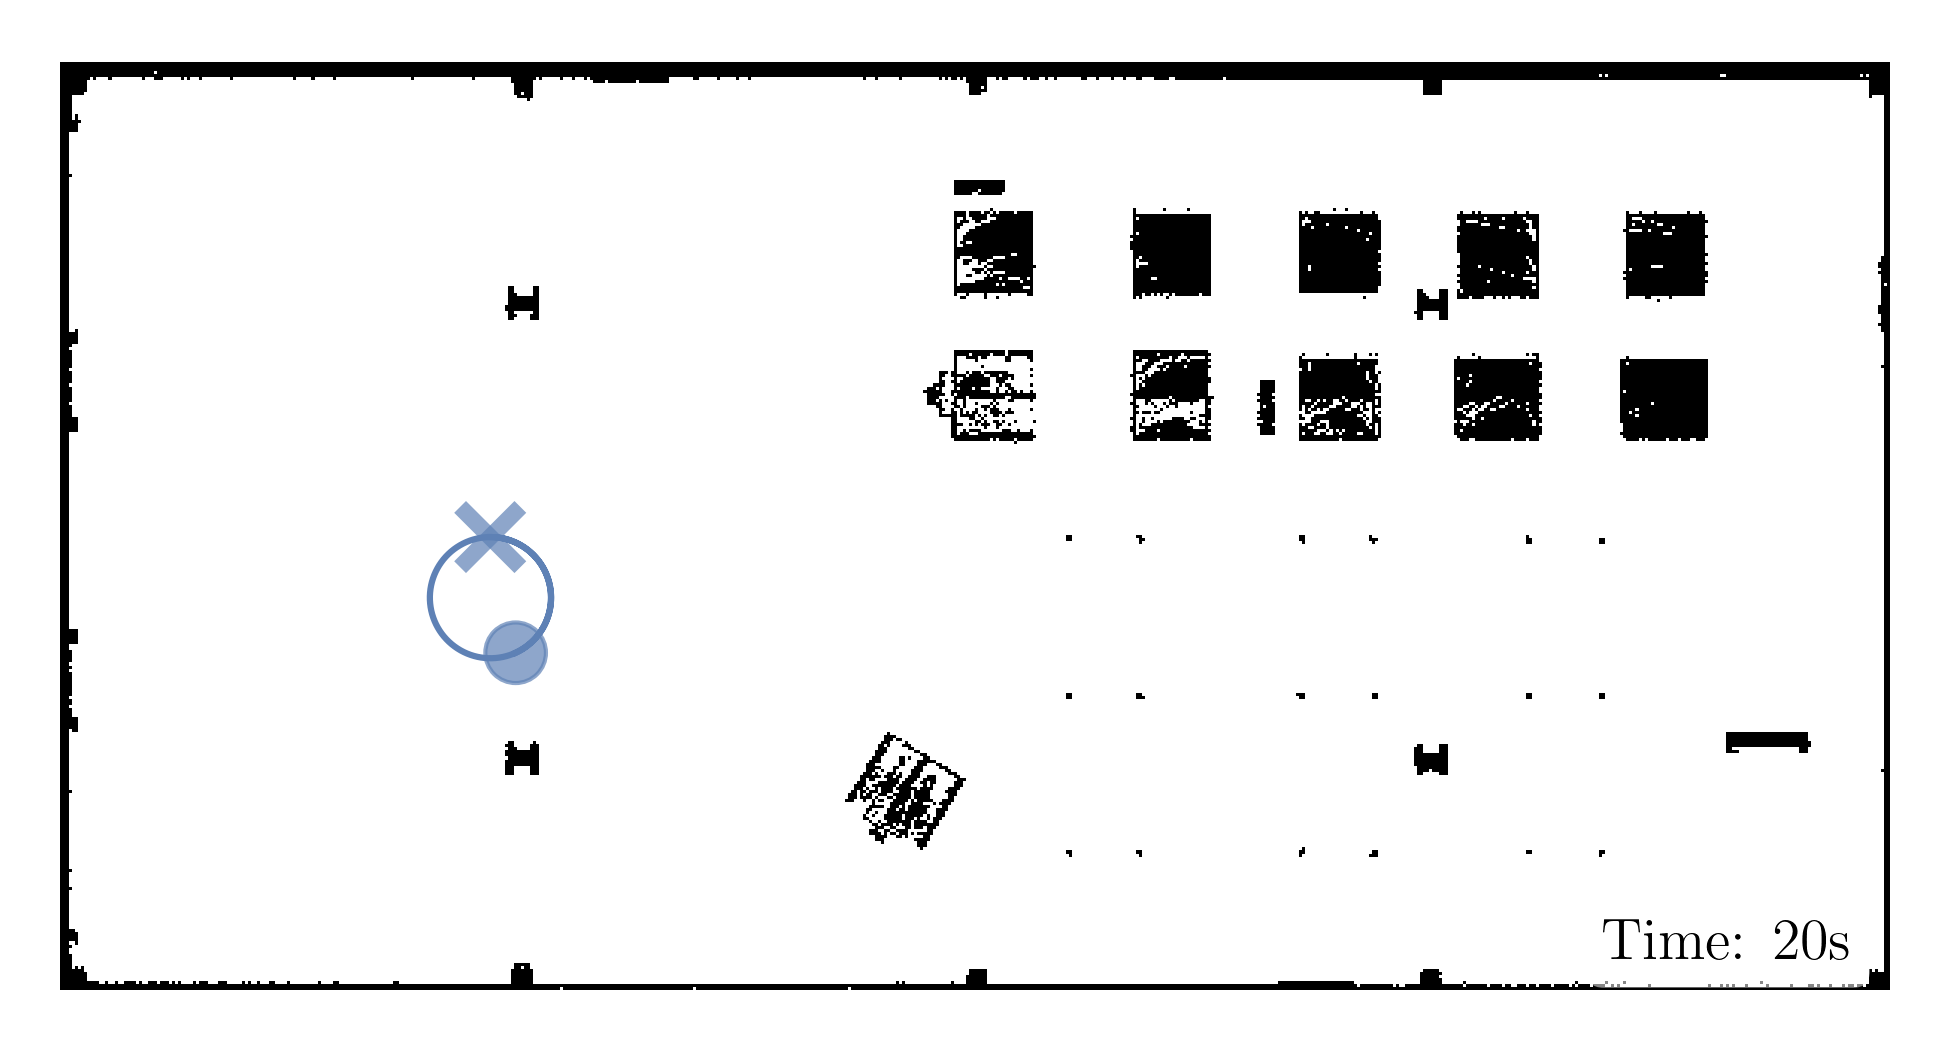
\includegraphics[width=\textwidth]{./figures/plots/consistency/simple-sim-paths-(after-20s).png}
    \caption{Simple Sim}
  \end{subfigure}
  \begin{subfigure}[b]{0.45\textwidth}
    \centering
    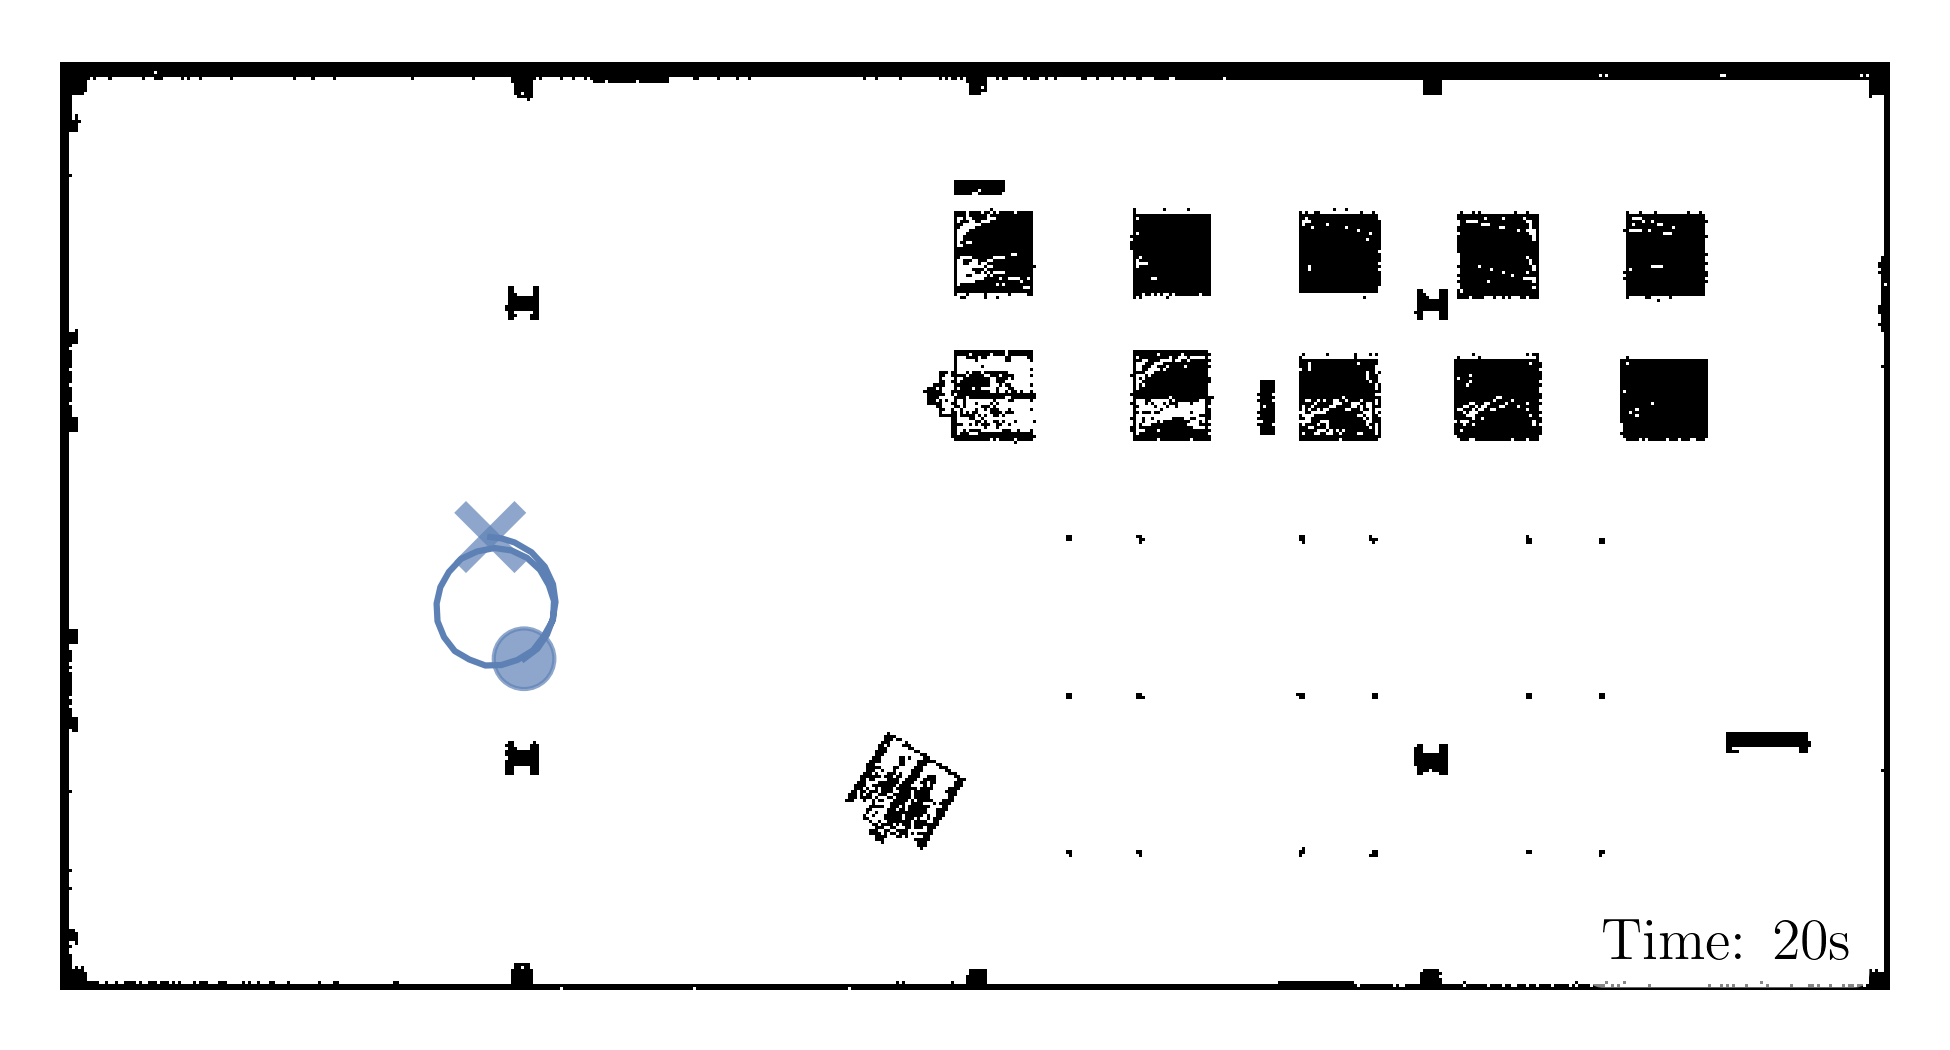
\includegraphics[width=\textwidth]{./figures/plots/consistency/ros-2-paths-(after-20s).png}
    \caption{ROS 2 Gazebo}
  \end{subfigure}
  \caption{Path when running circular behavior in \texttt{simple\_sim} and ROS 2 Gazebo.}
  \label{fig:movement-consistency}
\end{figure}

\subsubsection{Pathing}
% FIX: Change this text
A more complex evaluation was performed by comparing the main search behaviors. 
As shown in \cref{fig:coverage-benchmark-all}, the coverage curves produced by each simulator are closely aligned, particularly in early and mid-stage exploration. 
Minor deviations are attributed to non-determinism in Gazebo and slight differences in physics and sensor modeling.

The expectation is that the differences in the Gazebo and \texttt{simple\_sim} coverage over time, see \cref{fig:coverage-benchmark-diff}, will be consistent between the different search behaviors.


% TODO: Update this with new
\begin{figure}[H]
  \centering
  \begin{tabular}{cc}
    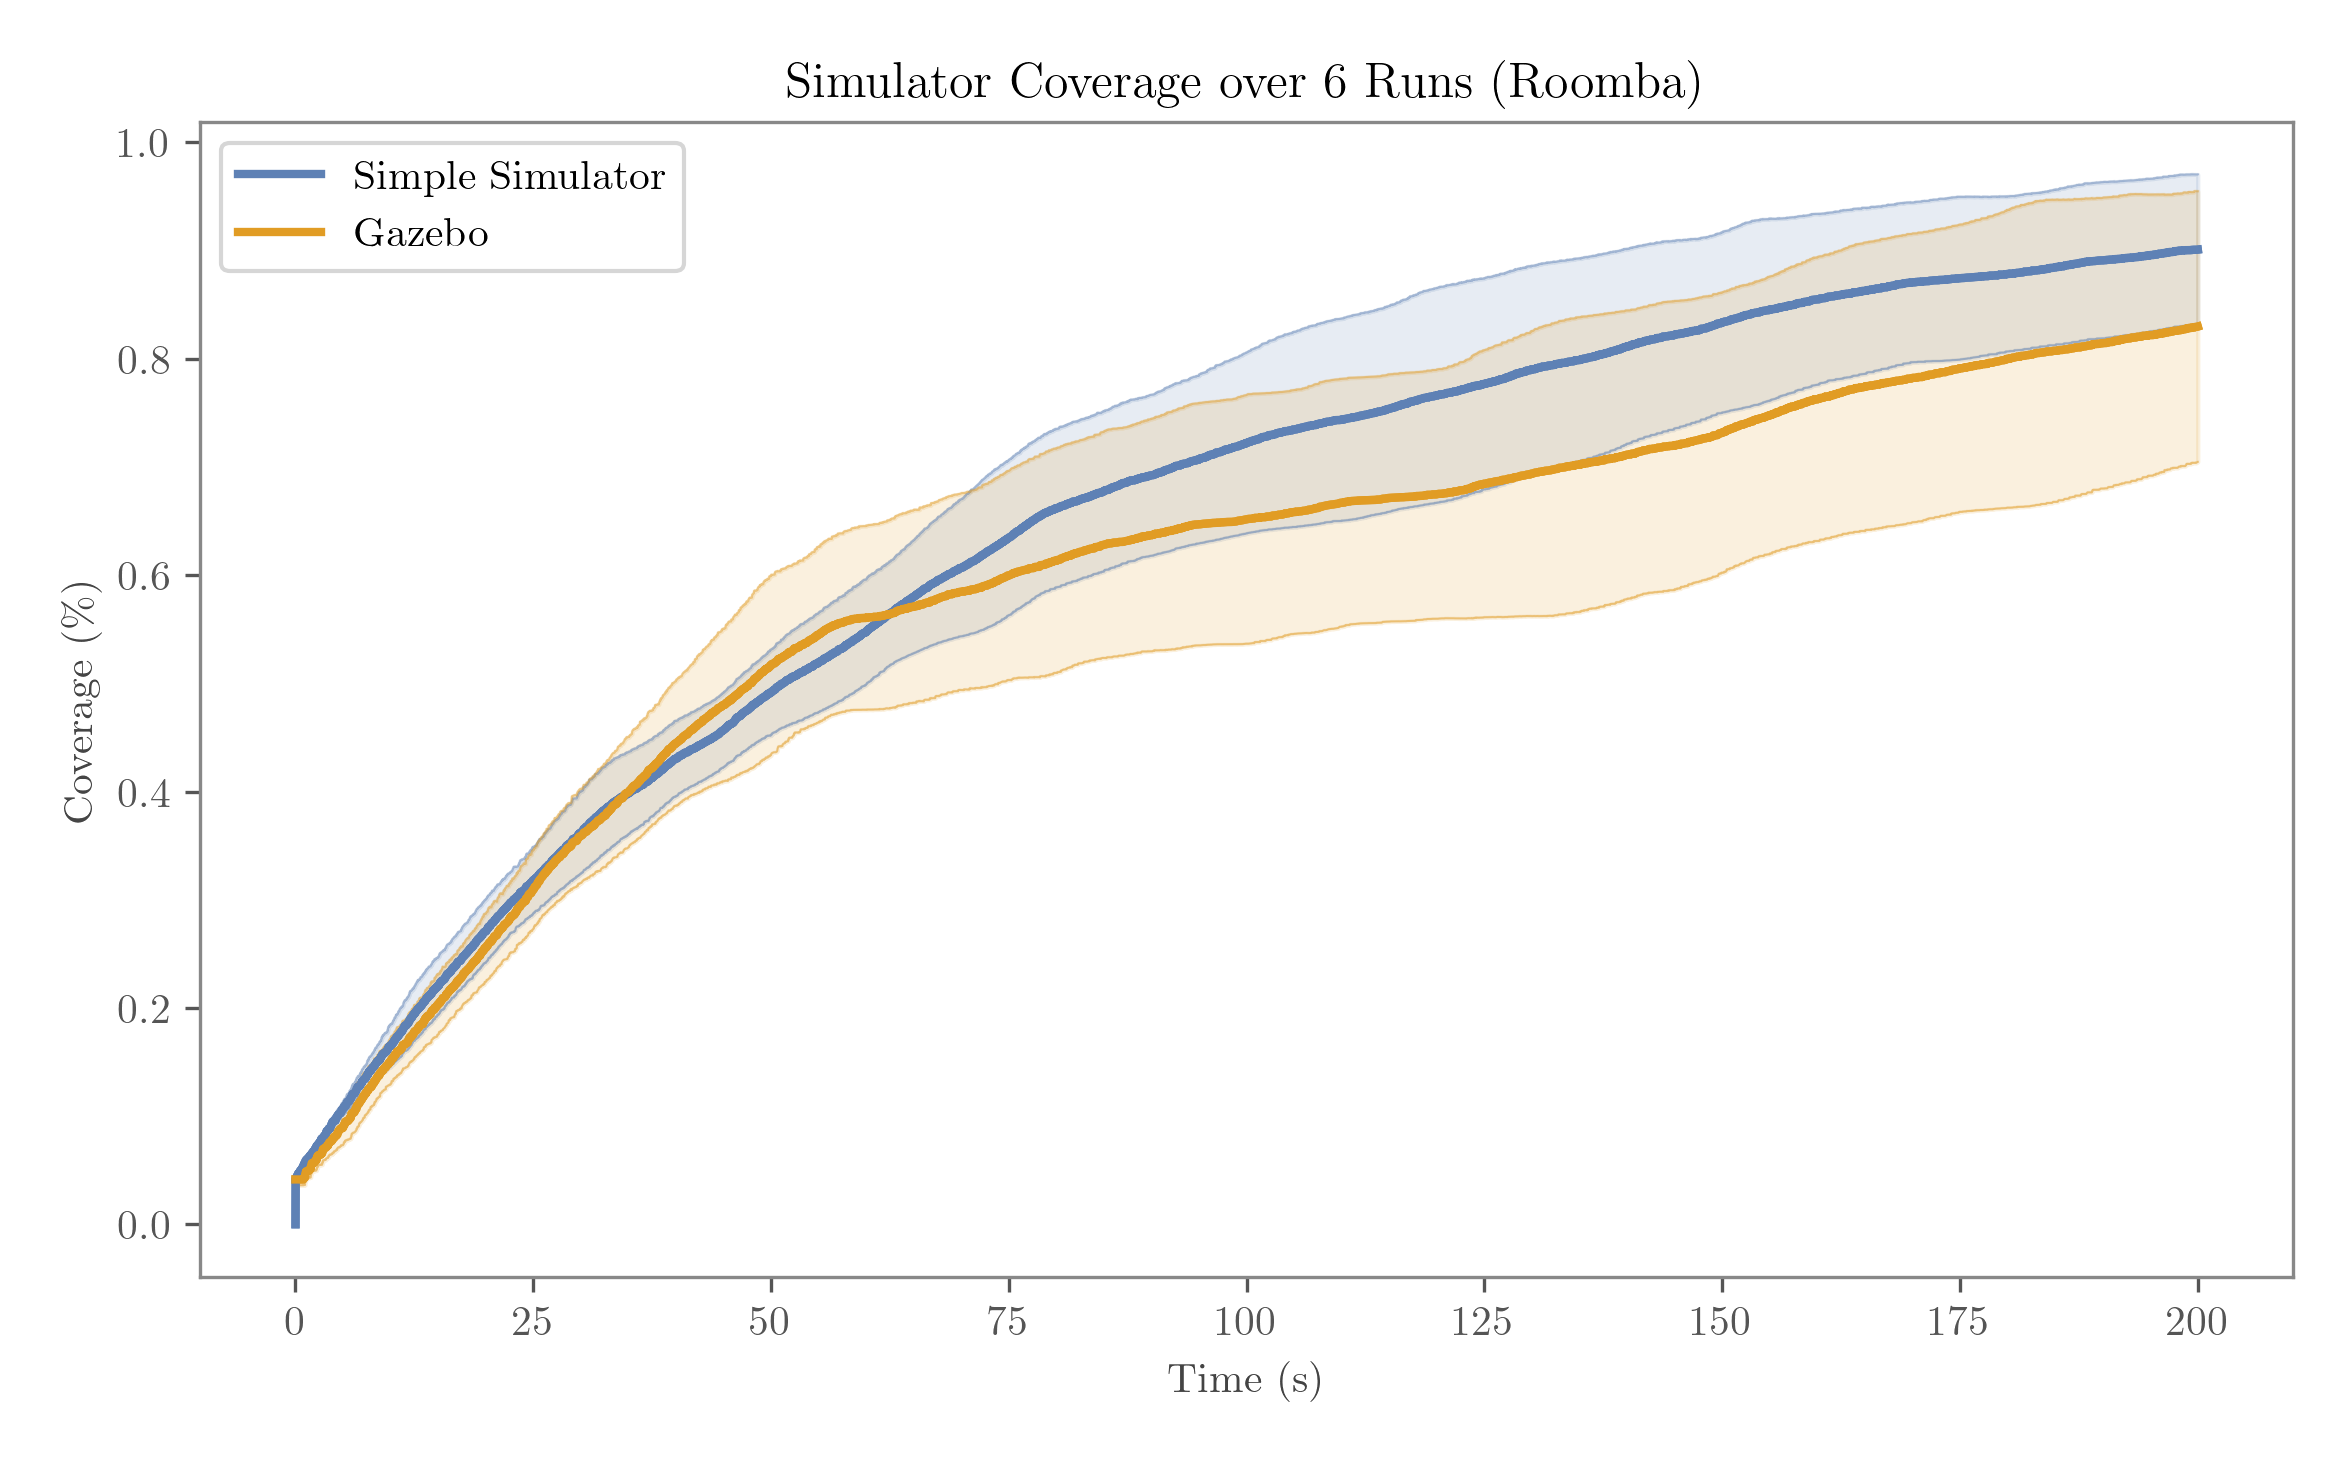
\includegraphics[width=0.45\textwidth]{./figures/plots/consistency/gazebo_vs_simple_sim_roomba.png} &
    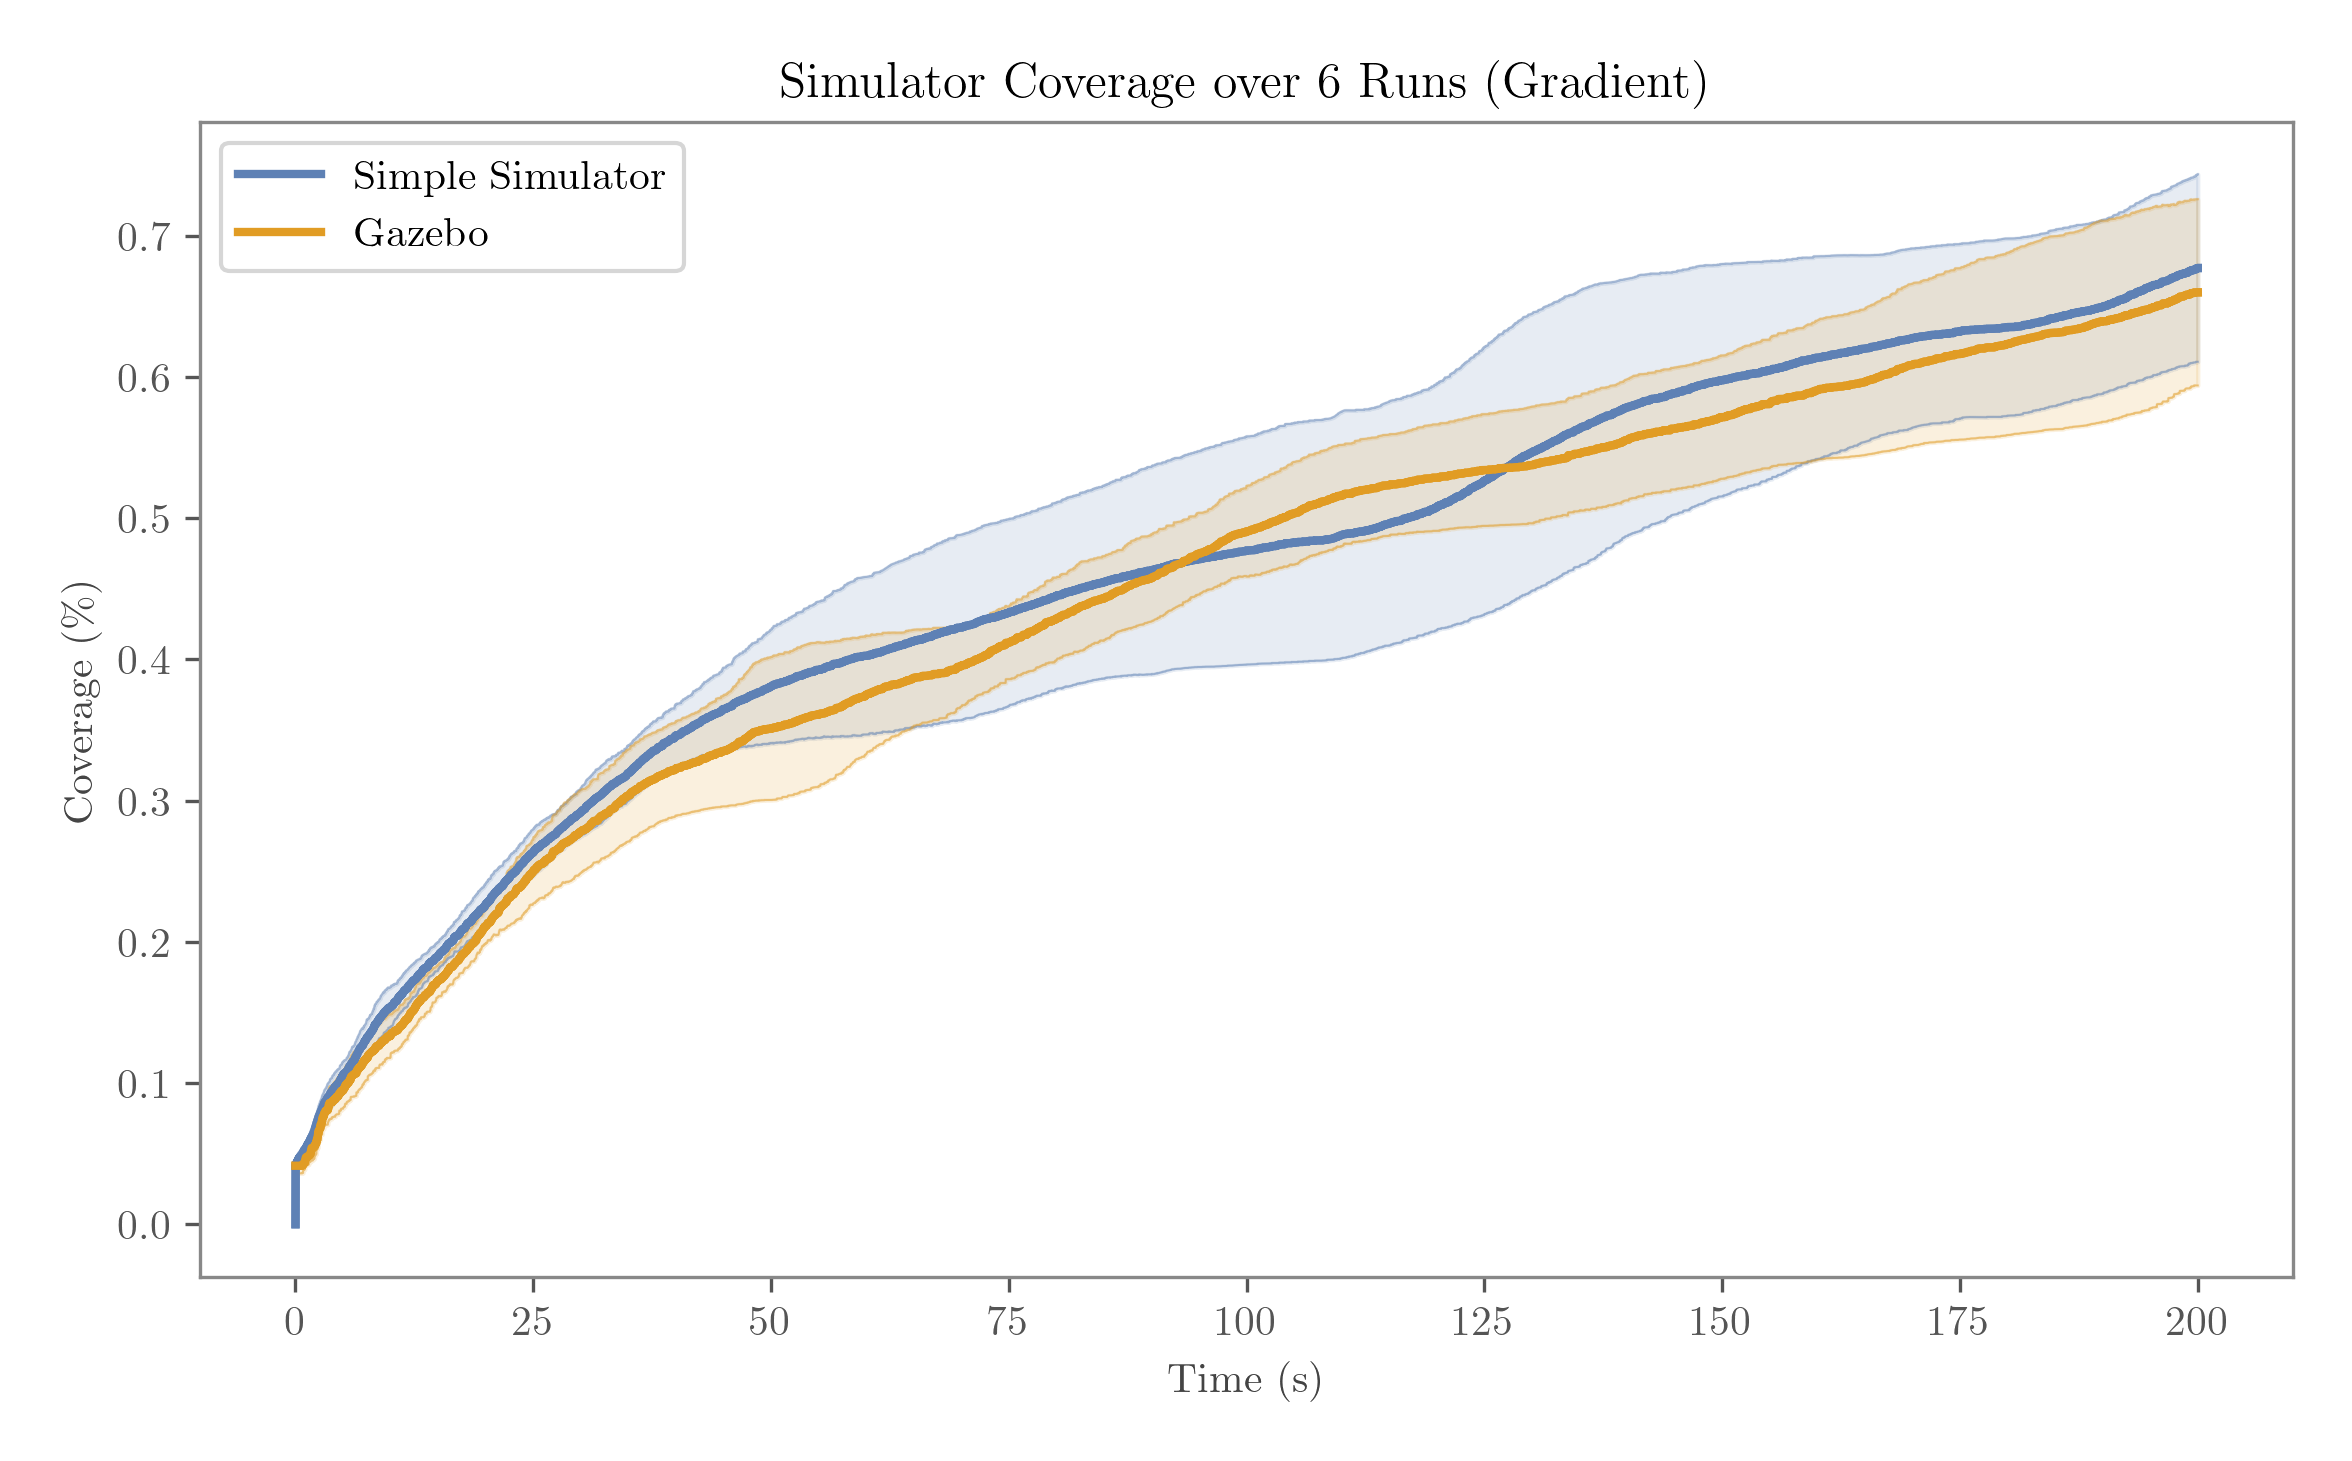
\includegraphics[width=0.45\textwidth]{./figures/plots/consistency/gazebo_vs_simple_sim_gradient.png} \\
    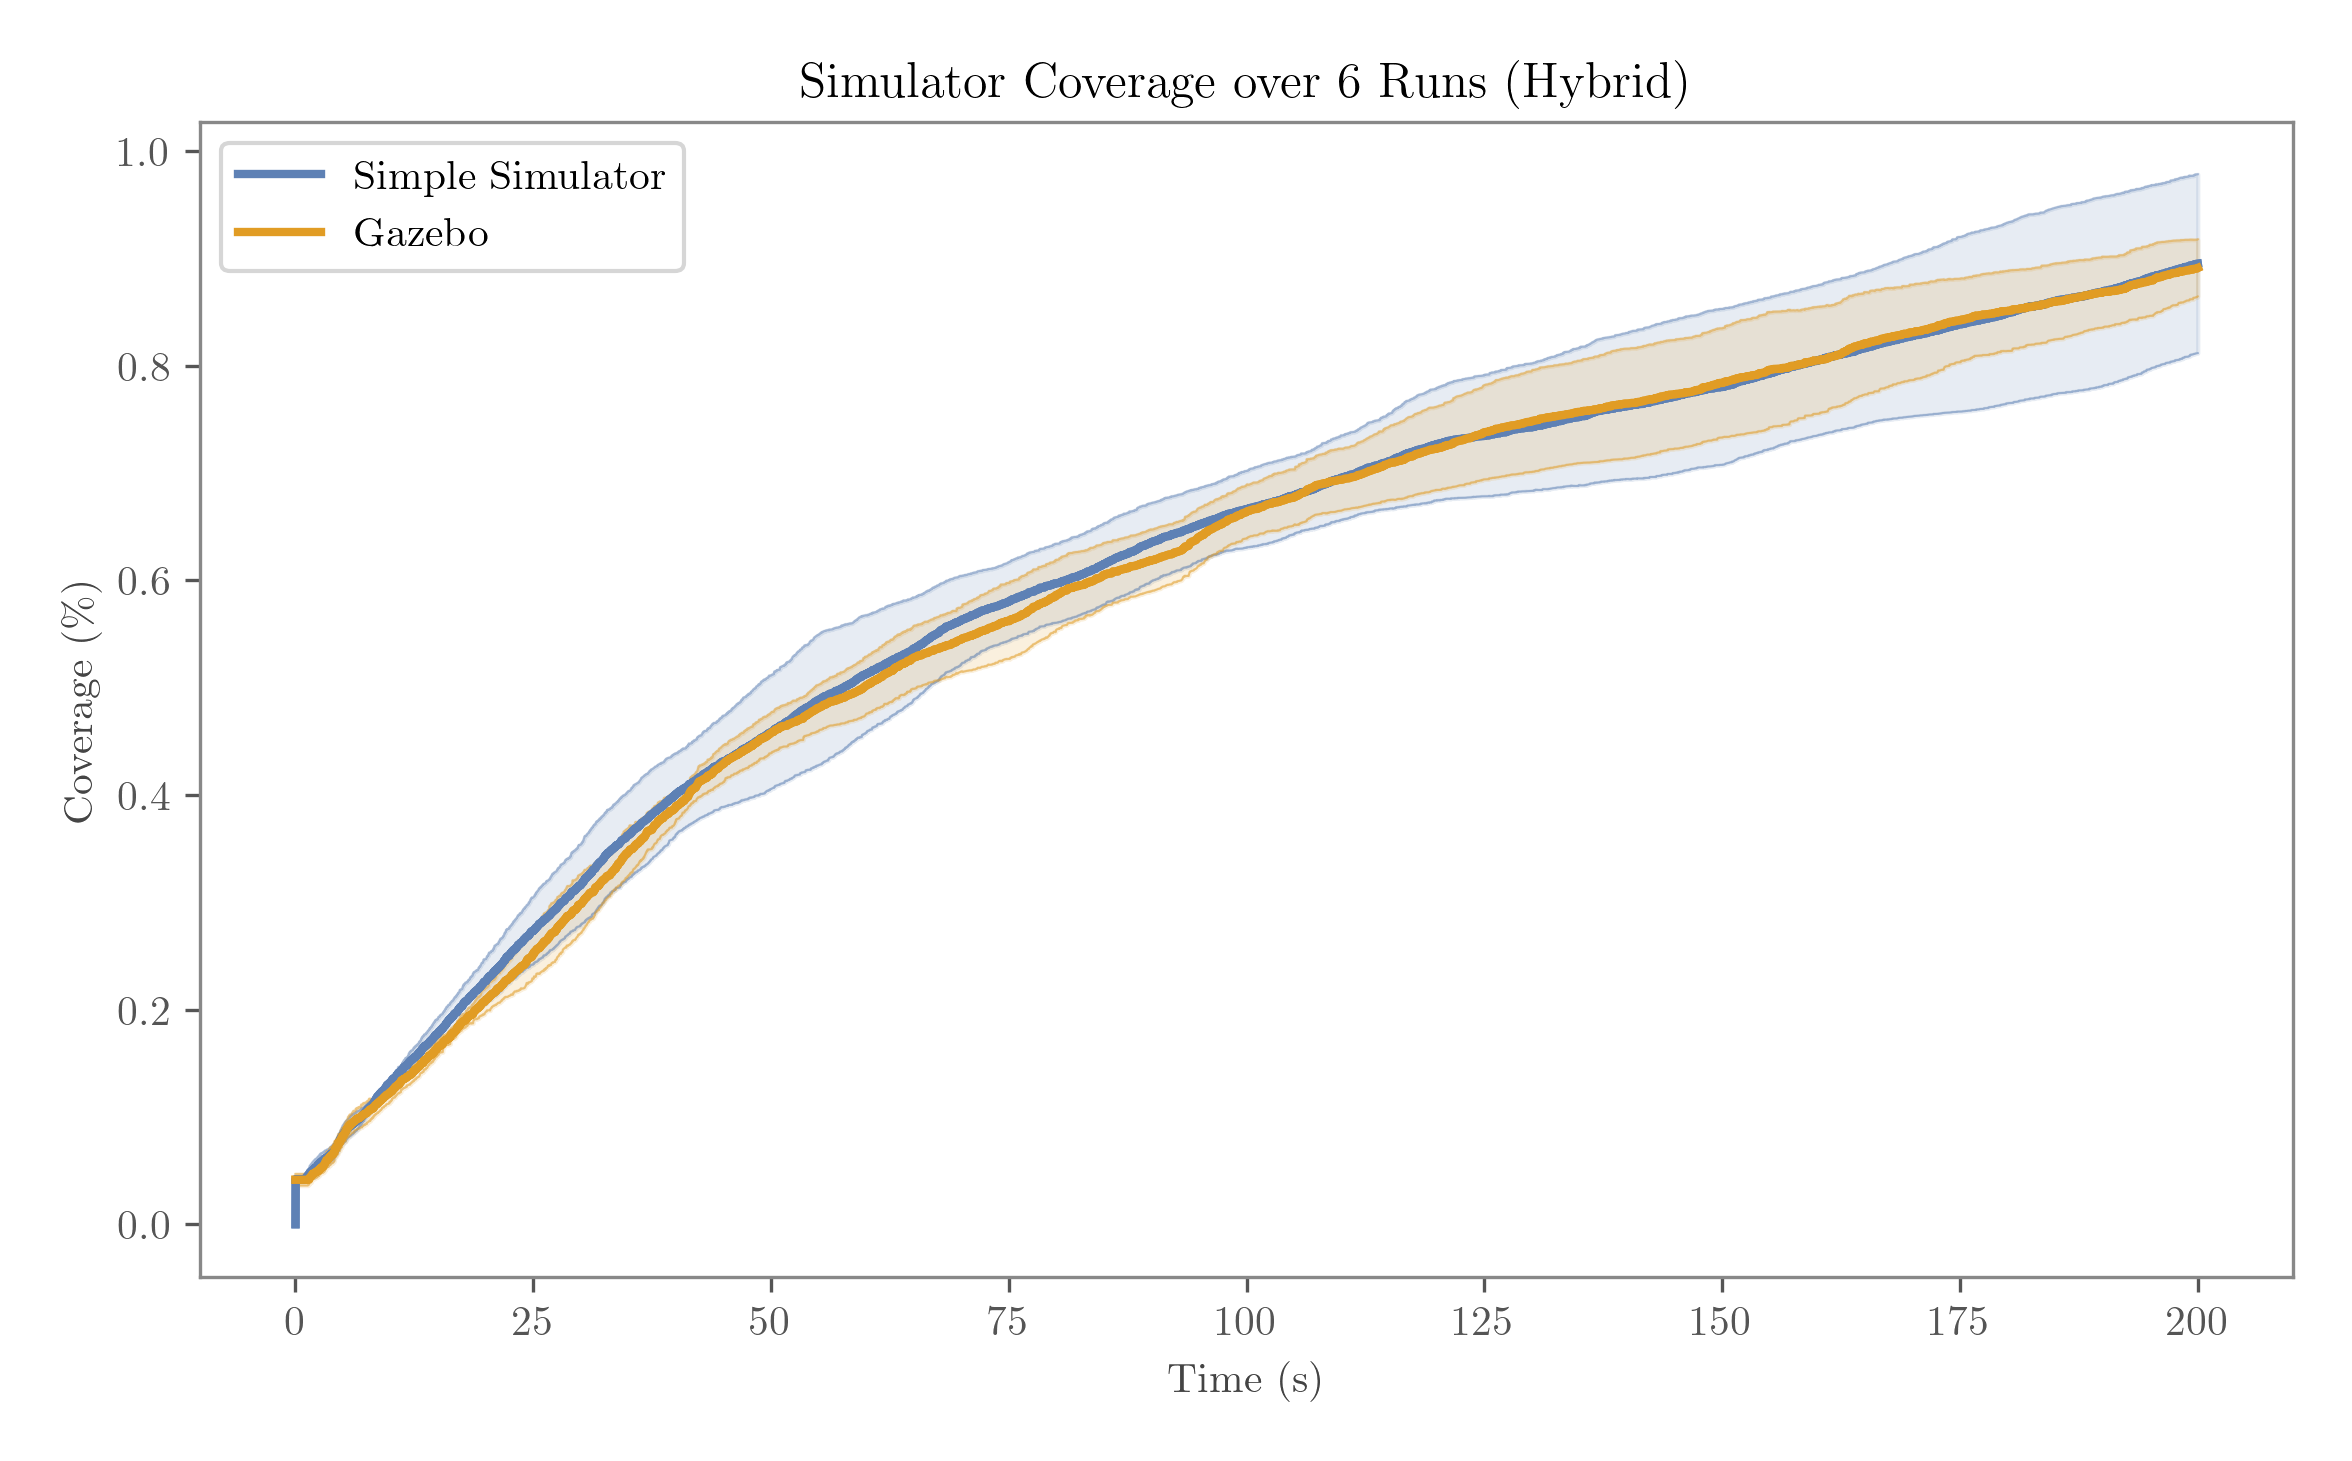
\includegraphics[width=0.45\textwidth]{./figures/plots/consistency/gazebo_vs_simple_sim_hybrid.png} &
    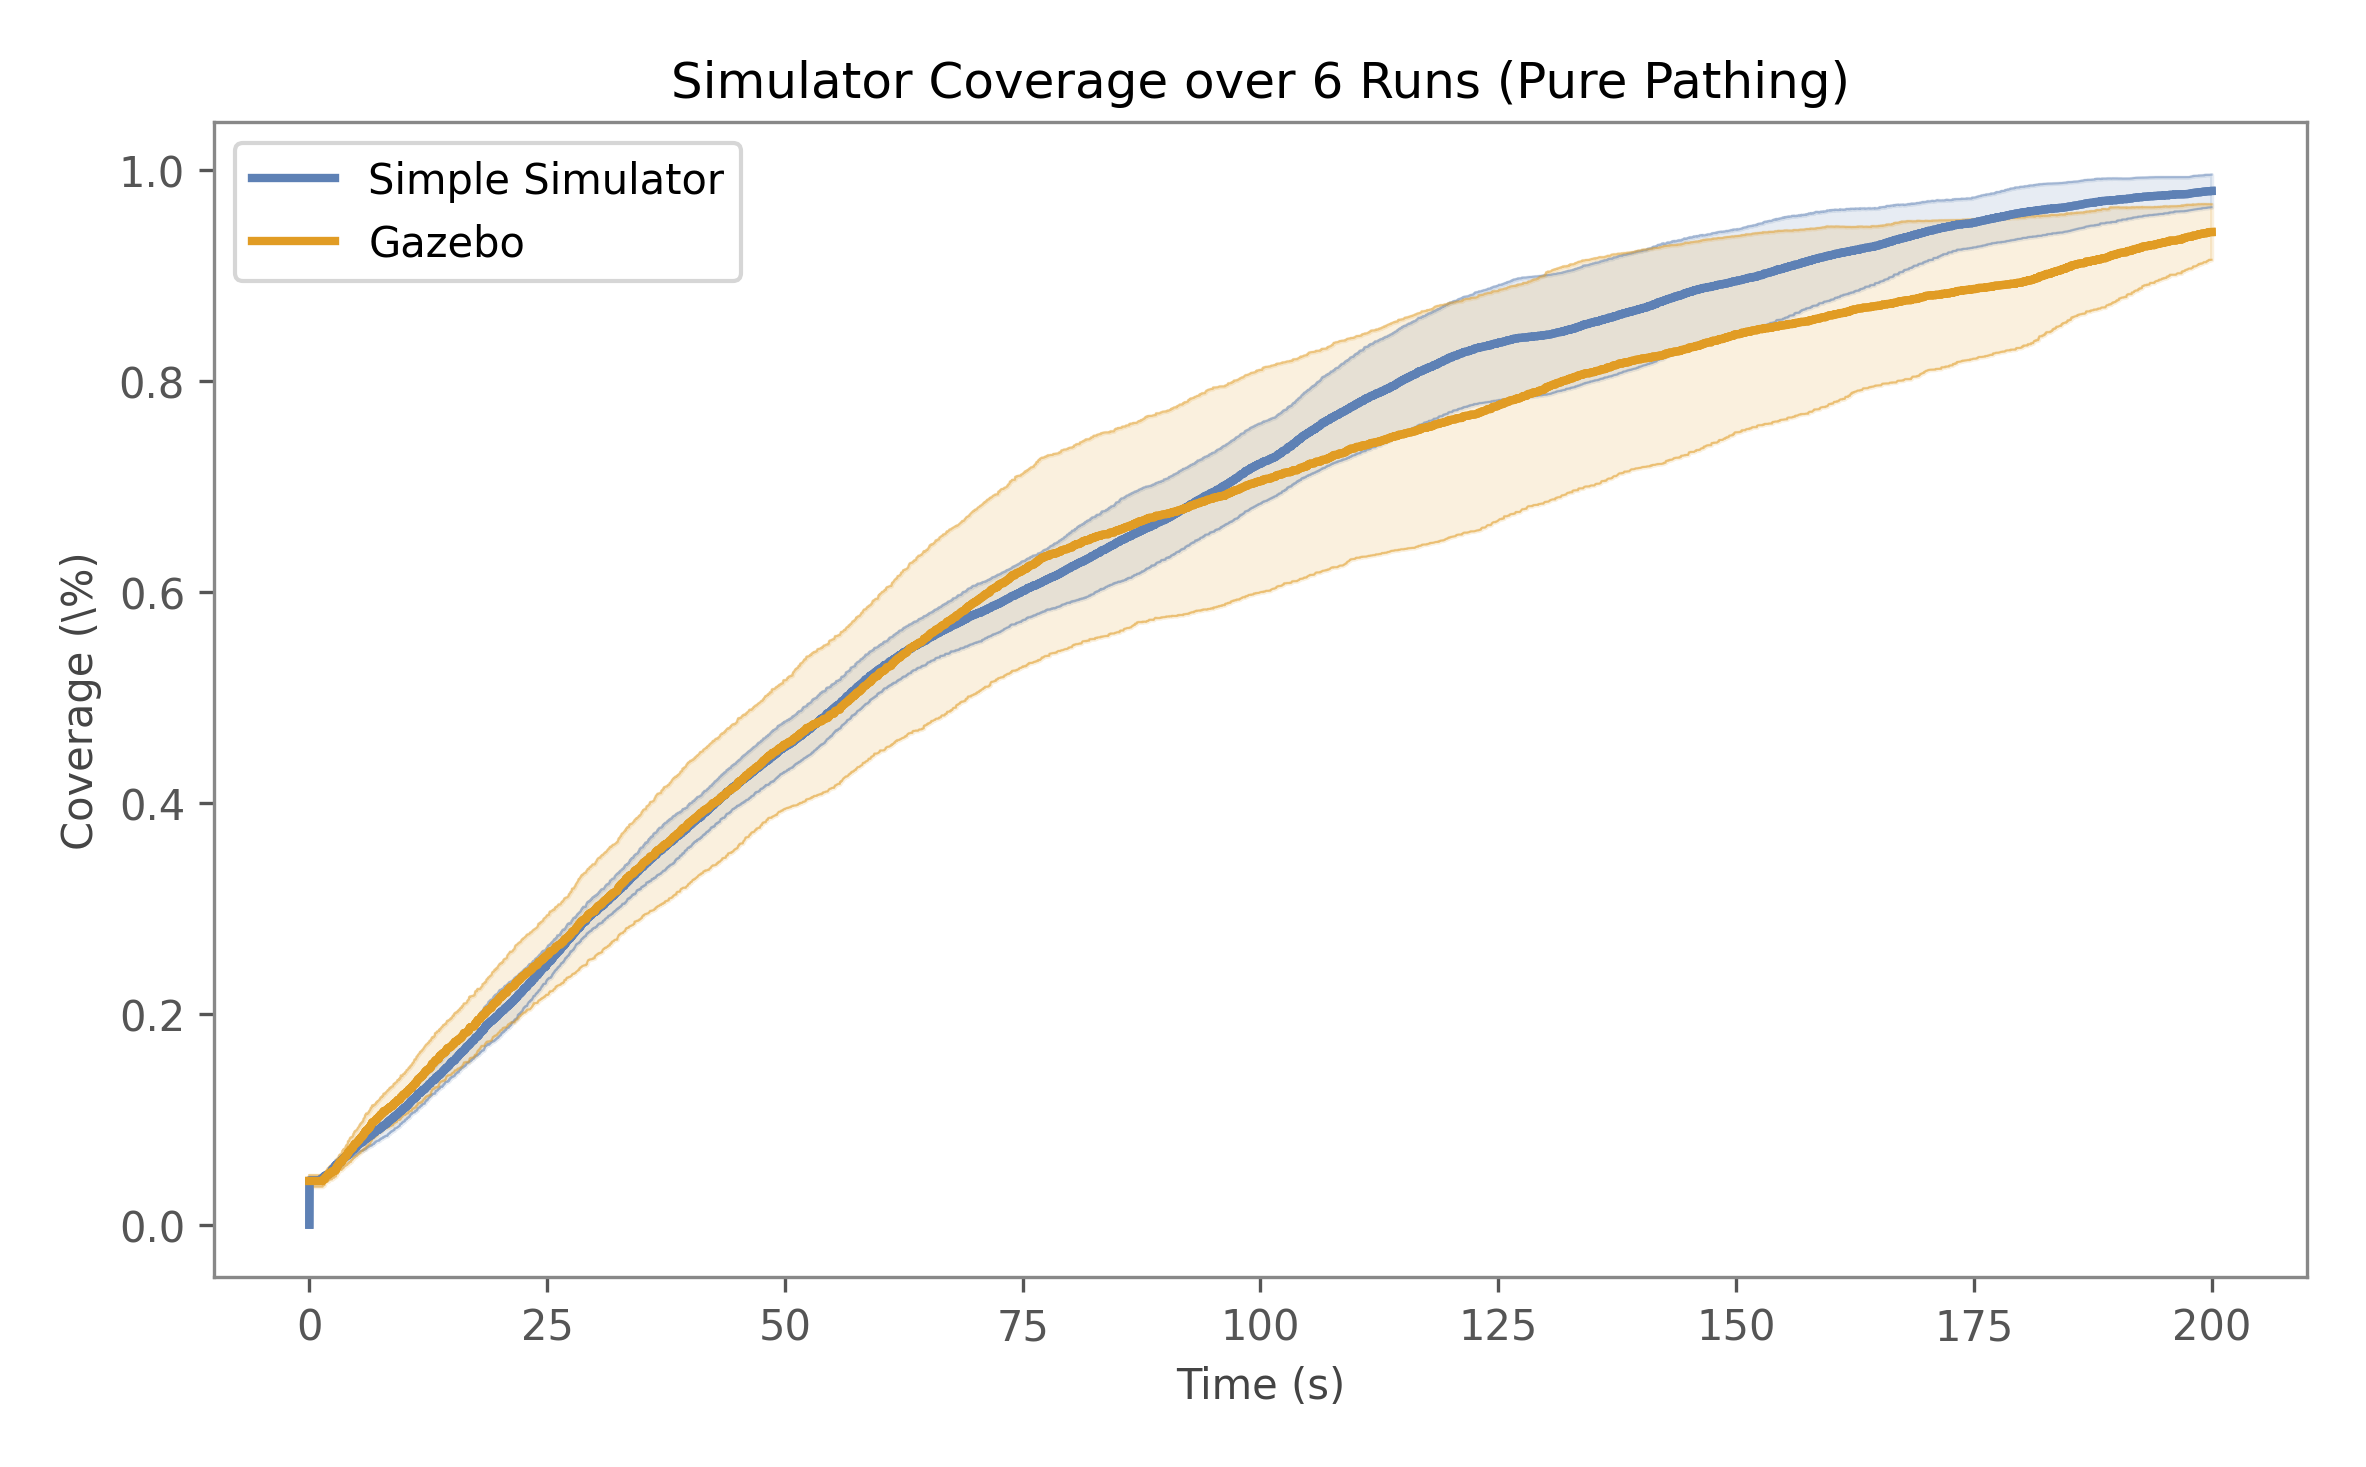
\includegraphics[width=0.45\textwidth]{./figures/plots/consistency/gazebo_vs_simple_sim_pure_pathing.png} \\
  \end{tabular}
  \caption{Comparison of coverage with spread over time between ROS 2 Gazebo and \texttt{simple\_sim}.}
  \label{fig:coverage-benchmark-all}
\end{figure}

% TODO: Update this with new
\begin{figure}[H]
    \begin{center}
        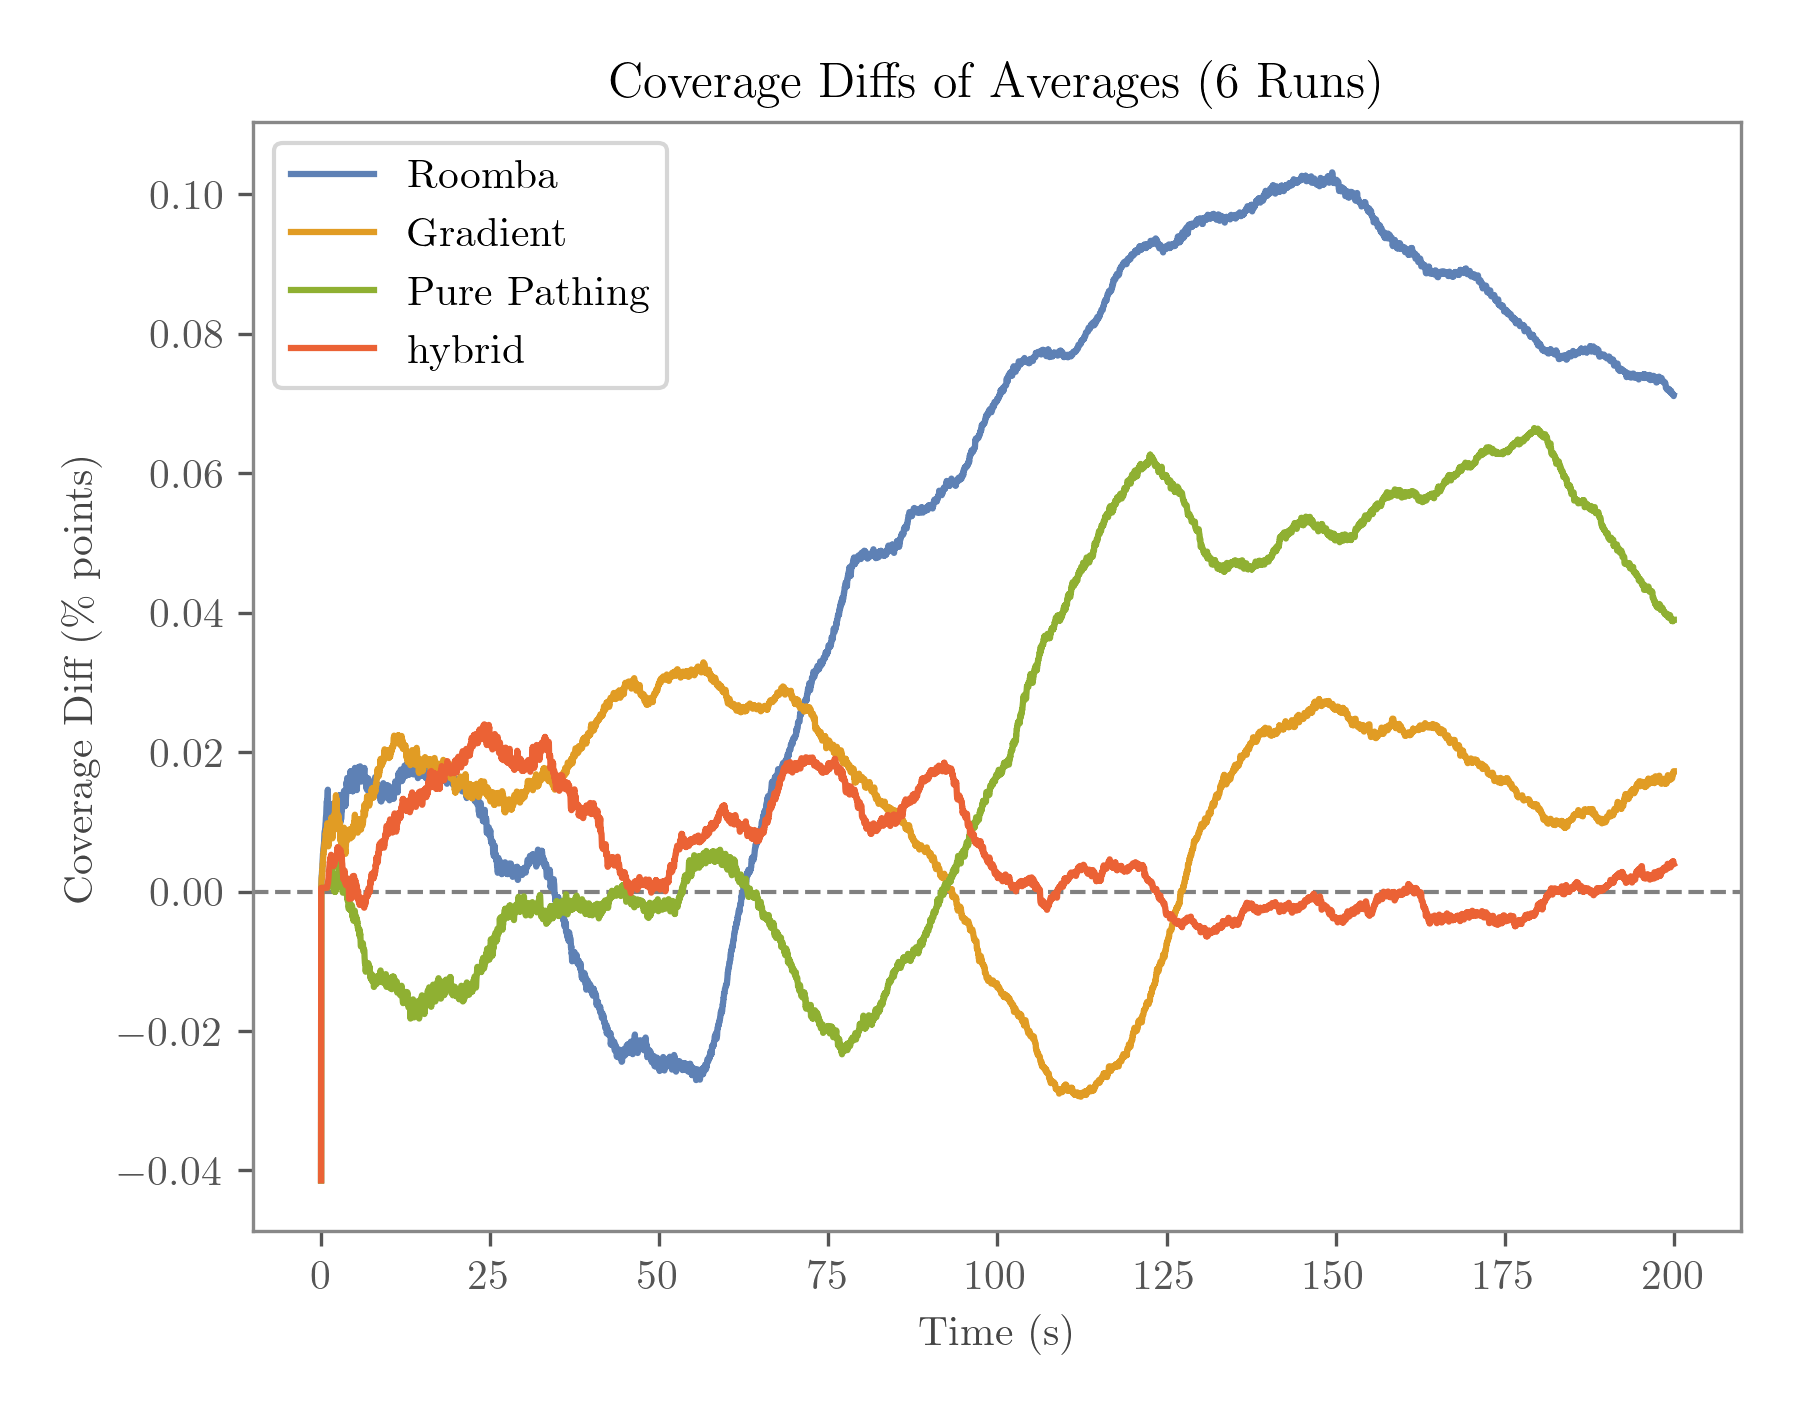
\includegraphics[width=0.75\textwidth]{./figures/plots/consistency/coverage-diffs-of-averages-(6-runs).png}
    \end{center}
    \caption{Comparison of difference in coverage over time between ROS 2 Gazebo and \texttt{simple\_sim}.}
    \label{fig:coverage-benchmark-diff}
\end{figure}

\subsection{Search Algorithm Benchmarks}
To evaluate search efficiency, each algorithm was executed across multiple randomly generated maps. The benchmark shown in \cref{fig:search-coverage-benchmark} presents average coverage over 10 runs, along with minimum and maximum bounds for each time step.

\begin{figure}[H]
    \begin{center}
        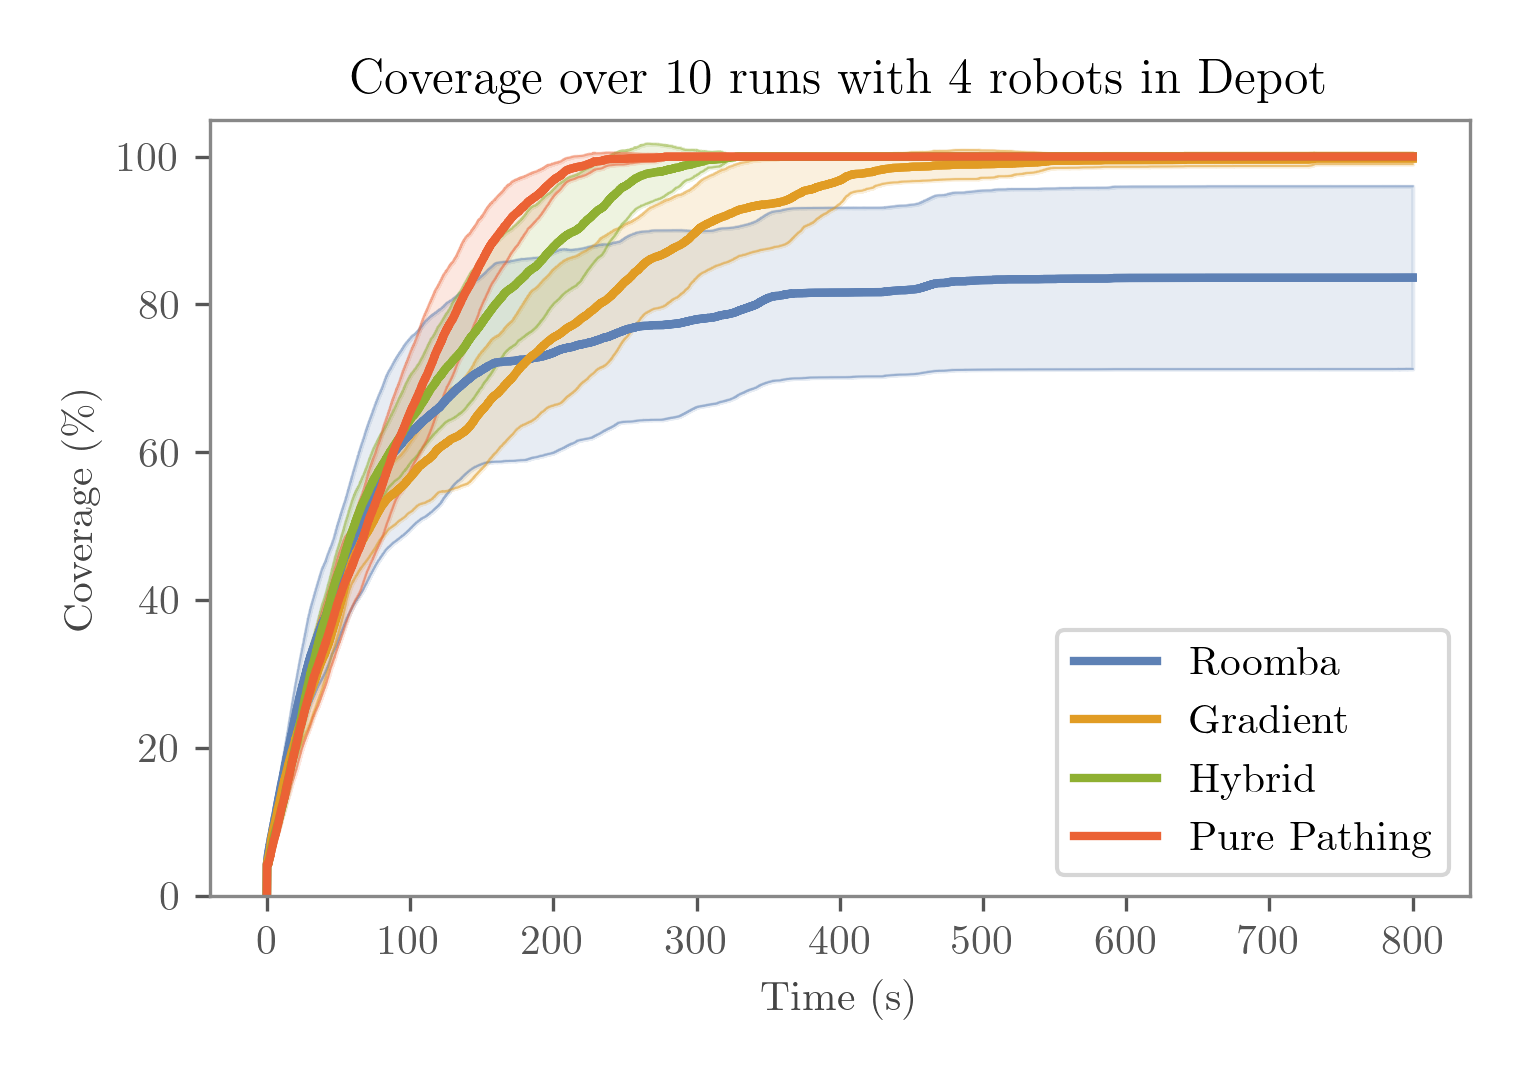
\includegraphics[width=0.95\textwidth]{./figures/plots/benchmarks/coverage-over-10-runs-with-4-robots-in-depot.png}
    \end{center}
    \caption{Coverage performance of search algorithms over 10 runs starting in random positions in the same environment. Shaded regions represent the range between minimum and maximum coverage at each time step.}
    \label{fig:coverage-benchmark}
\end{figure}

All algorithms eventually achieve full coverage, though their exploration efficiency varies significantly. 
Gradient-based methods tend to cover local areas quickly but slow down due to diminishing gradients near fully explored zones. 
Frontier-based methods achieve higher global efficiency by directing robots toward unknown regions, but at a higher computational cost. The hybrid method strikes a balance by switching strategies based on local exploration progress. 
Deep reinforcement learning shows promise but requires further tuning for consistent early-stage performance.

\subsection{Performance}
A critical aspect of the performance of the search algorithms is computational and communication requirement for running the behaviors. 
\subsubsection{Computation Time}
% FIX: Mean line not working
% TODO: Maybe change from ms pr step to percent comparison with roomba as baseline
% TODO: State Average time for each algorithm
\cref{fig:computation-performance} shows the computation time for each algorithm on the same map. As expected the Roomba algorithm is the fastest but the other is not quite as expected.
The Pure Pathing algorithm is the next fastest, when not including the outliers. 
This is due to the path following being very cheap and only the generation of the costmap, frontier exploration, and frontier evaluation being expensive. 
The expensive operations does not occur frequently enough to significantly impact the average computation time.
\begin{figure}[H]
    \begin{center}
        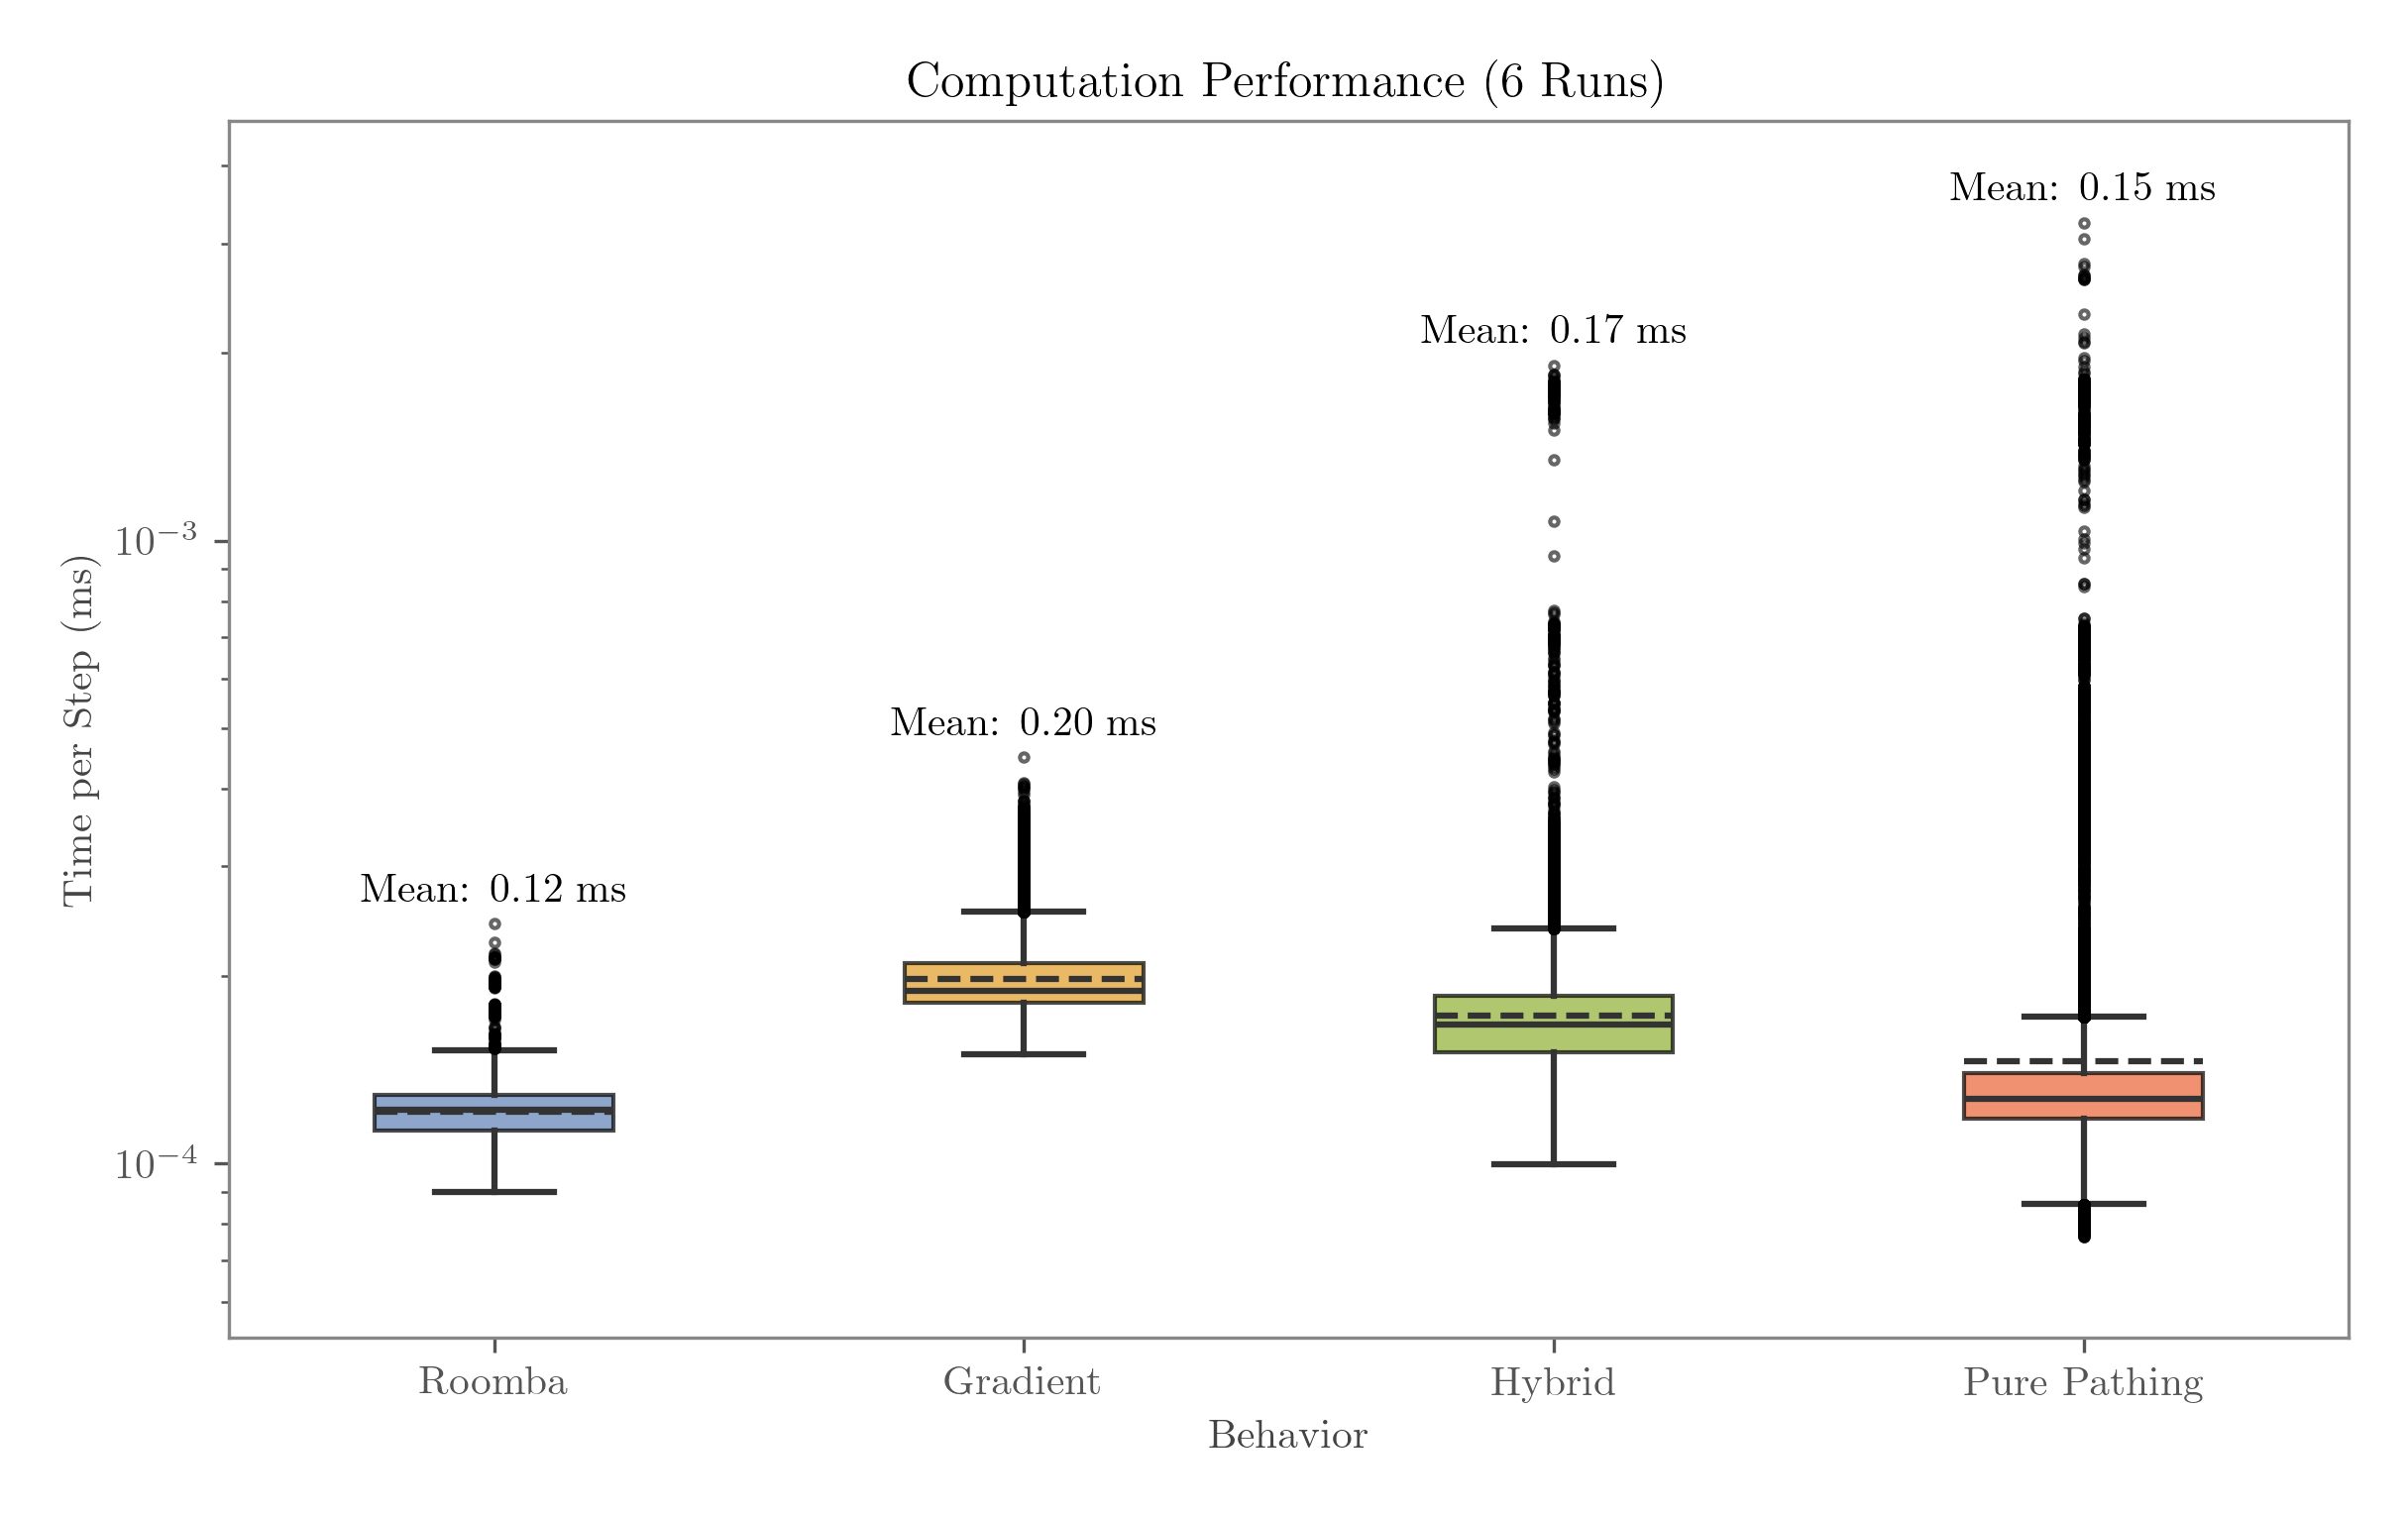
\includegraphics[width=0.75\textwidth]{./figures/plots/computation-performance-(6-runs).png}
    \end{center}
    \caption{Computation time box plot for each algorithm on the same map.}
    \label{fig:computation-performance}
\end{figure}

\subsubsection{Communication {\color{red}Load}}
\begin{figure}[H]
    \begin{center}
        \includegraphics[width=0.75\textwidth]{./figures/plots/bytes.png}
    \end{center}
    \caption{Message size boxplot for each algorithm on the same map.}
    \label{fig:computation-performance}
\end{figure}
